\chapter{Условие}%
\label{cha:uslovie}

\section{Задача 1}%
\label{sec:task_1}
Для локальной общей сети был выделен частный адрес 192.168.x.0/24

Разделить сеть на 5 подсетей
\begin{enumerate}
    \item Подсети 1 и 5 должны поддерживать до x + 10 устройств

    \item Подсети 2 и 4 должны поддерживать до 5 устройств

    \item Подсеть 3 должна поддерживать только 2 устройства
\end{enumerate}
Где x - Ваш номер по списку в ЭУ

Использовать не более трех подсетей с возможностью размещения x + 10 хостов

\section{Задача 2}%
\label{sec:task_2}

Настроить DHCP-сервера для выдачи адресов
\begin{enumerate}
    \item Для подсети 1 настроить отдельный DHCP сервер
    \item Для подсети 2 настроить в качестве DHCP-сервера маршрутизатор 1
    \item Для подсетей 4 и 5 настроить в качестве DHCP-сервера маршрутизатор 2
\end{enumerate}

\chapter{Практическая часть}%
\label{cha:prakticheskaia_chast_}

\section{Разделение ip-адресов на подсети}%
\label{sec:1}
\begin{table}[H]
    \centering
    \caption{Разделение на подсети}
    \label{tab:networks}
    \begin{tabular}{|p{0.8cm}|p{1cm}|p{3cm}|p{3cm}|p{3cm}|p{3.2cm}|}
        \hline
        Но-мер под-се-ти & Ко-ли-чест-во хос-тов & ip подсети & Диапазон адресов & Широкове-щательный адрес & Маска под-сети \\
        \hline
        1 & 30 & 192.168.12.0 & 192.168.12.1-192.168.12.30 & 192.168.12.31 & 255.255.255.224 (/27) \\
        \hline
        2 & 6 & 192.168.12.64 & 192.168.12.65-192.168.12.70 & 192.168.12.71 & 255.255.255.248 (/29) \\
        \hline
        3 & 2 & 192.168.12.80 & 192.168.12.81-192.168.12.82 & 192.168.12.83 & 255.255.255.252 (/30) \\
        \hline
        4 & 6 & 192.168.12.72 & 192.168.12.73-192.168.12.78 & 192.168.12.79 & 255.255.255.248 (/29) \\
        \hline
        5 & 30 & 192.168.12.32 & 192.168.12.33-192.168.12.62 & 192.168.12.63 & 255.255.255.224 (/27) \\
        \hline
    \end{tabular}
\end{table}
\newpage
\section{Рабочай схема}%
\label{sec:work_schema}

\begin{figure}[htpb]
    \centering
    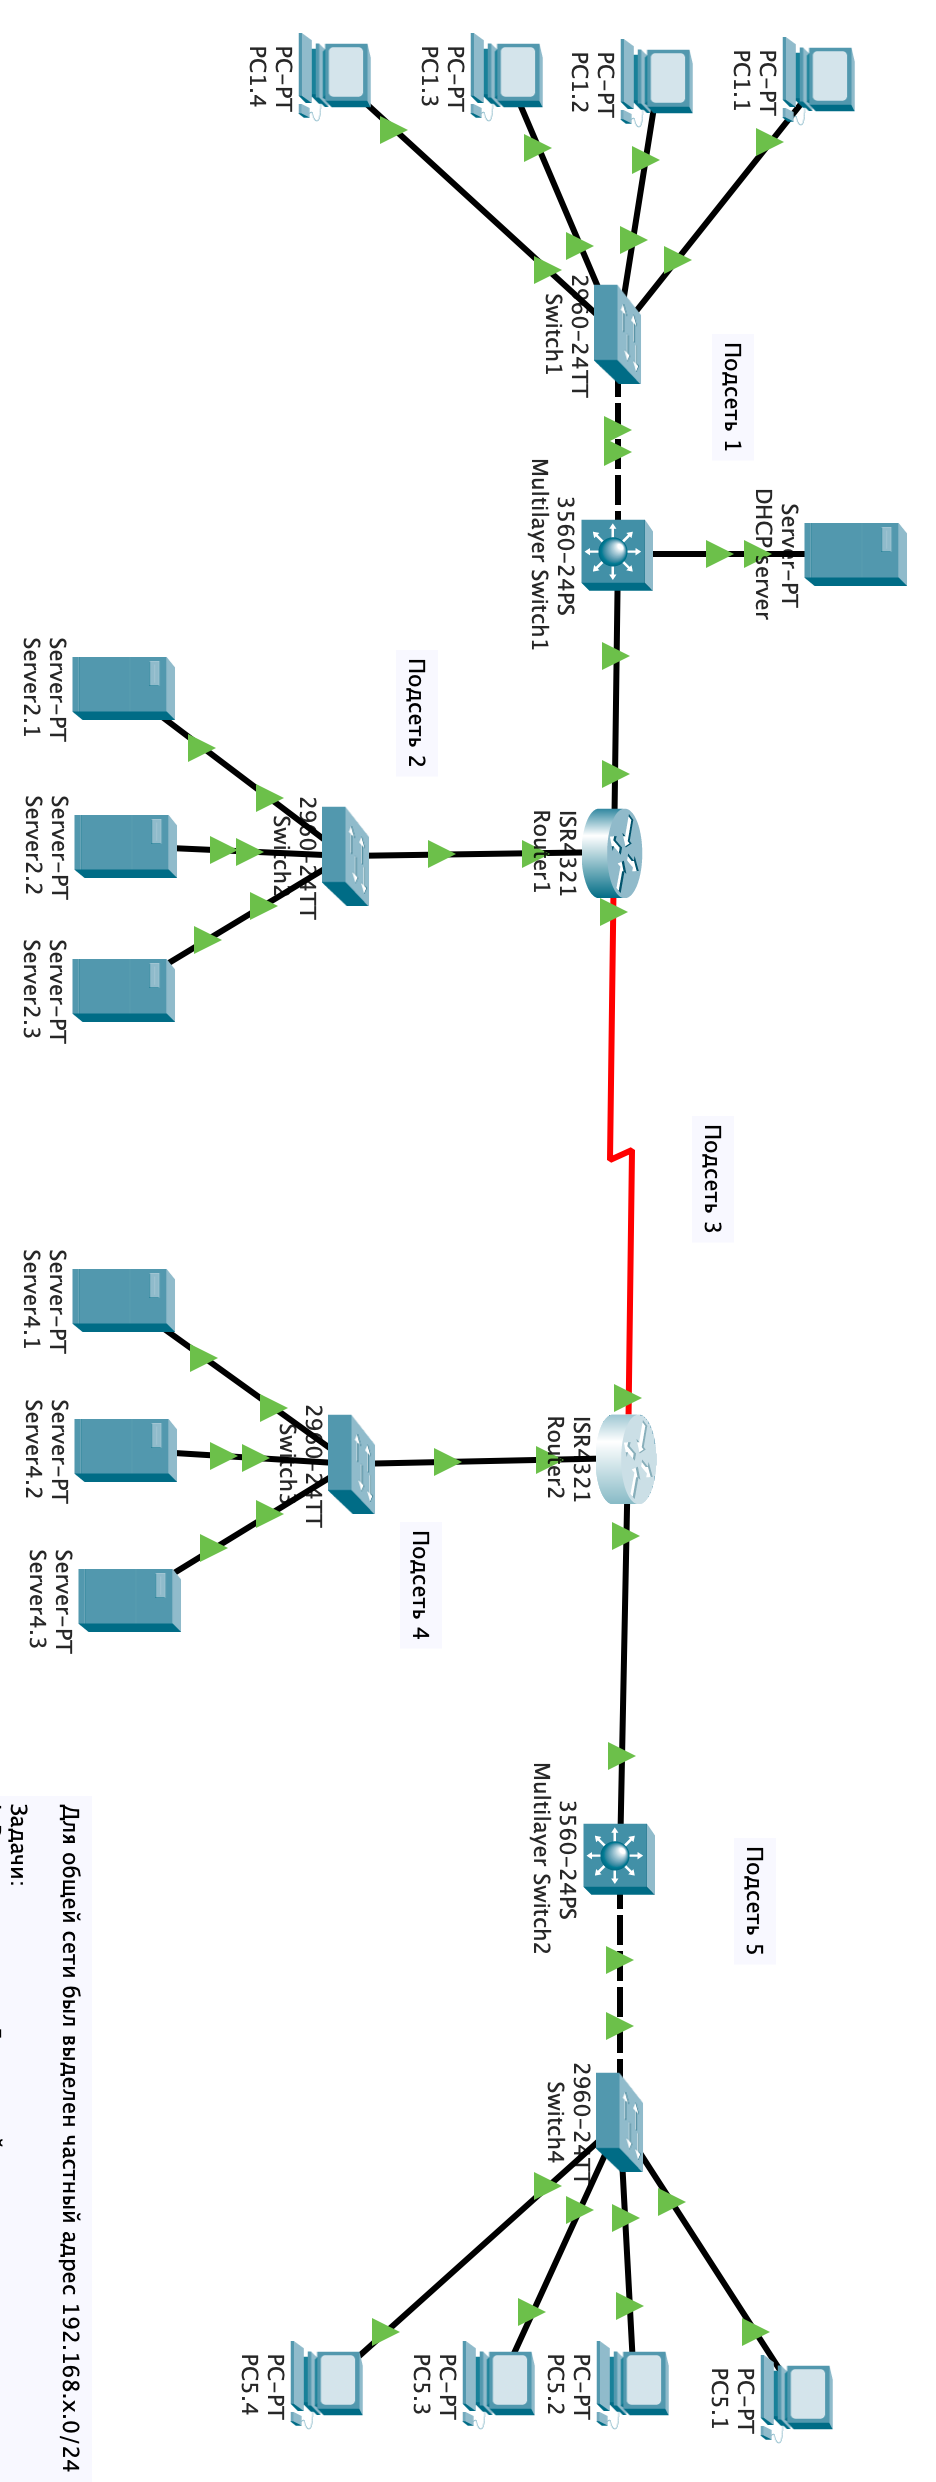
\includegraphics[width=0.4498\linewidth]{images/work_shema.png}
    \caption{Схема с настроенными подсетями}%
\end{figure}
\newpage

\section{Настройка DHCP-сервера для 1-ой подсети}%
\label{sec:1_net}

\begin{figure}[H]
    \centering
    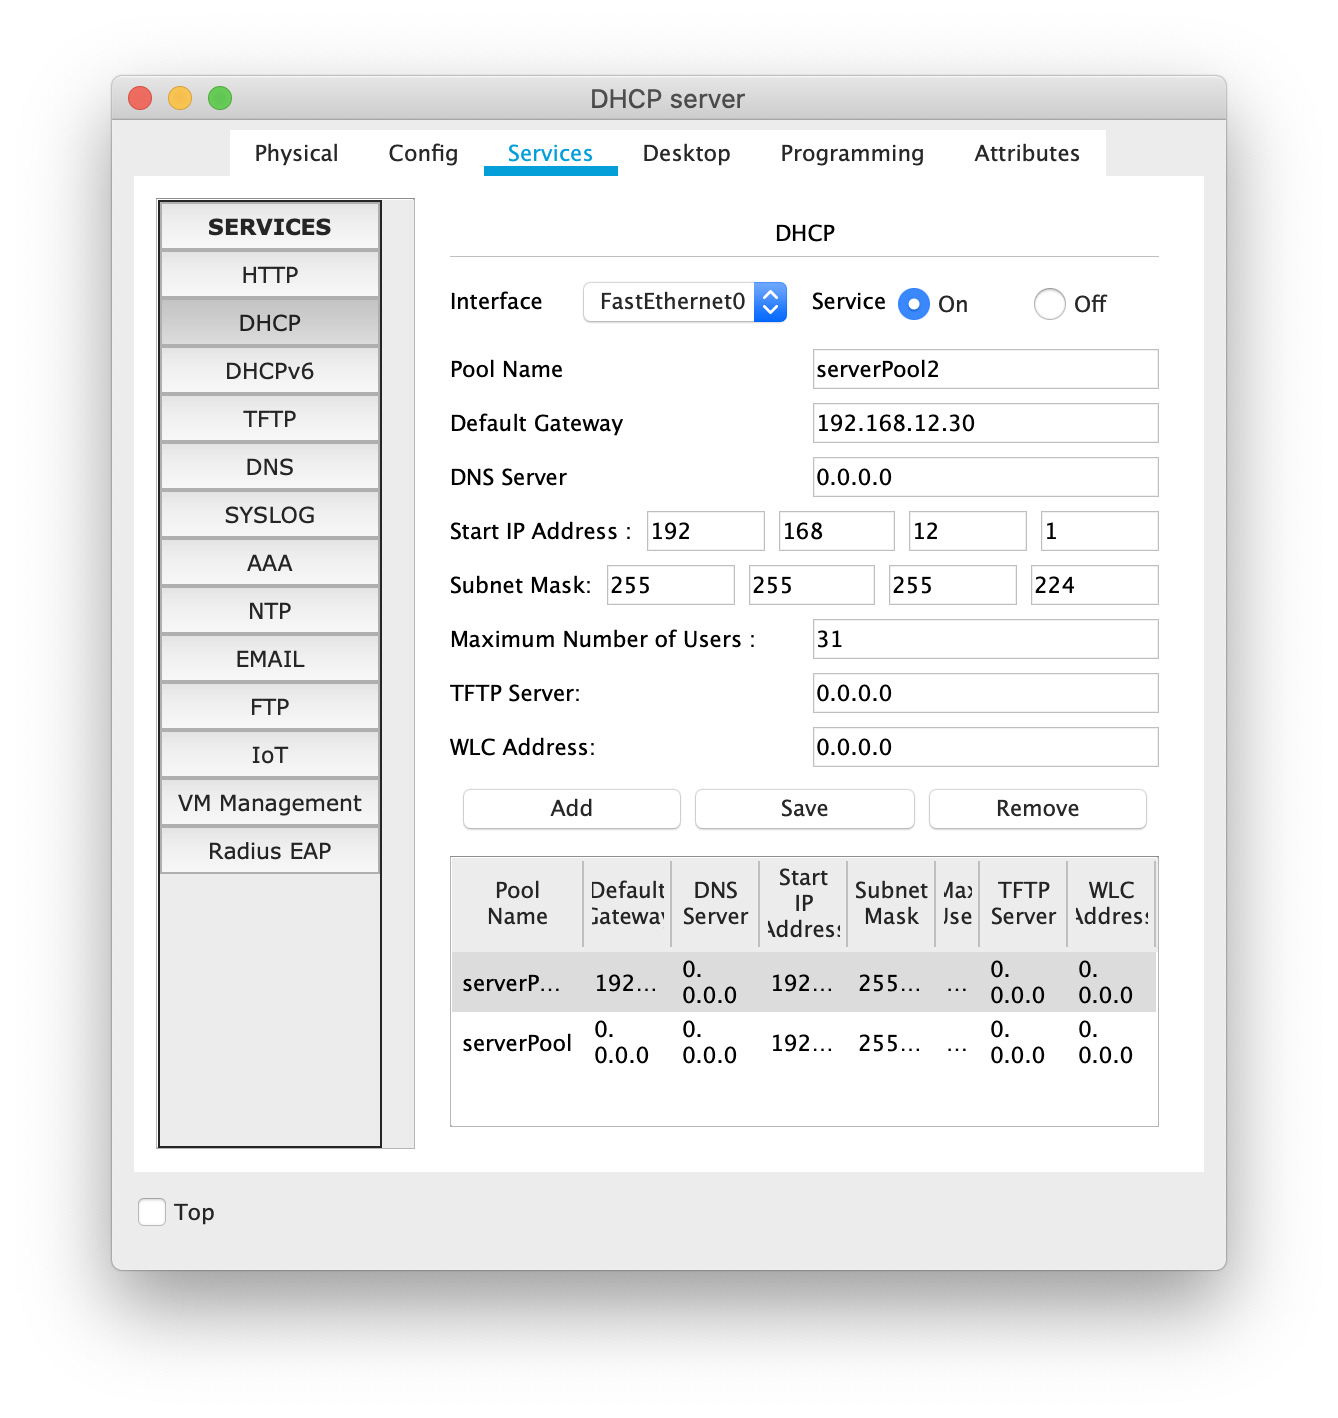
\includegraphics[width=0.7\linewidth]{images/dhcp_1.png}
    \caption{Настройка сервера}%
\end{figure}

IP-адреса конечным узлам в подсети выдаются автоматически из диапазона сетей подсети №1:

\begin{figure}[H]
    \centering
    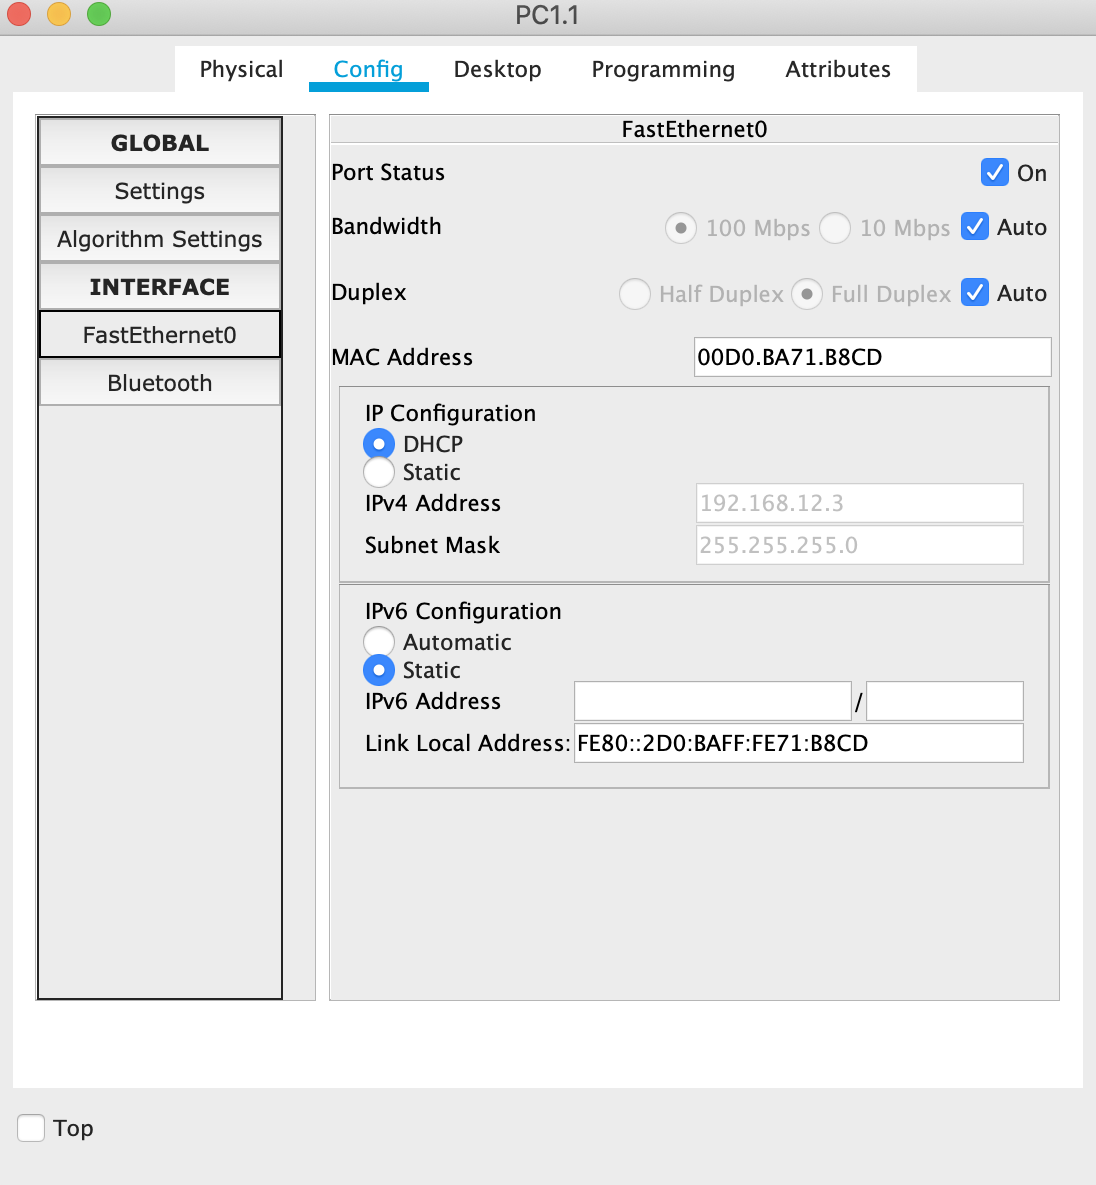
\includegraphics[width=0.7\linewidth]{images/net_1_machine.png}
    \caption{Автоматически выданный ip-адрес в первой подсети}%
\end{figure}


Проверка связи компьютеров в подсети №1:
\begin{figure}[H]
    \centering
    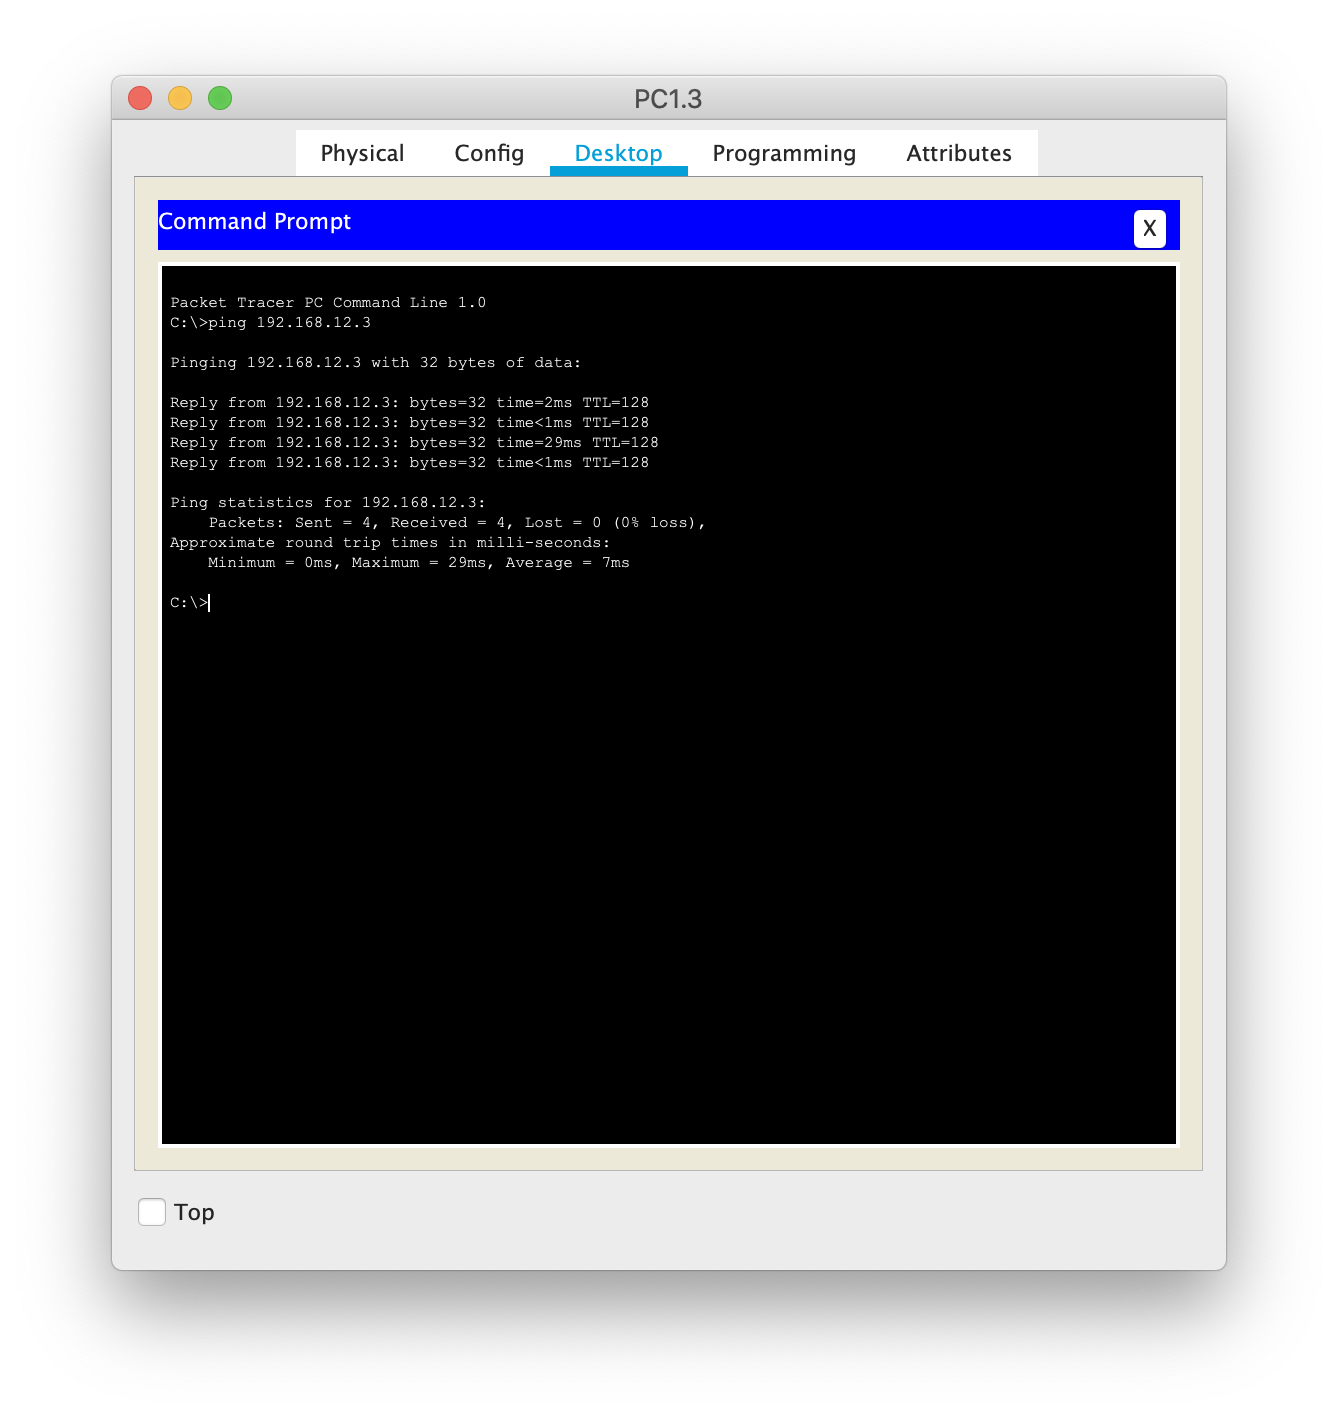
\includegraphics[width=0.8\linewidth]{images/net_1_ping.png}
    \caption{Результат использования ping}%
\end{figure}

\section{Настройка DHCP-сервера для 2-ой подсети}%
\label{sec:2_net}
\begin{figure}[H]
    \centering
    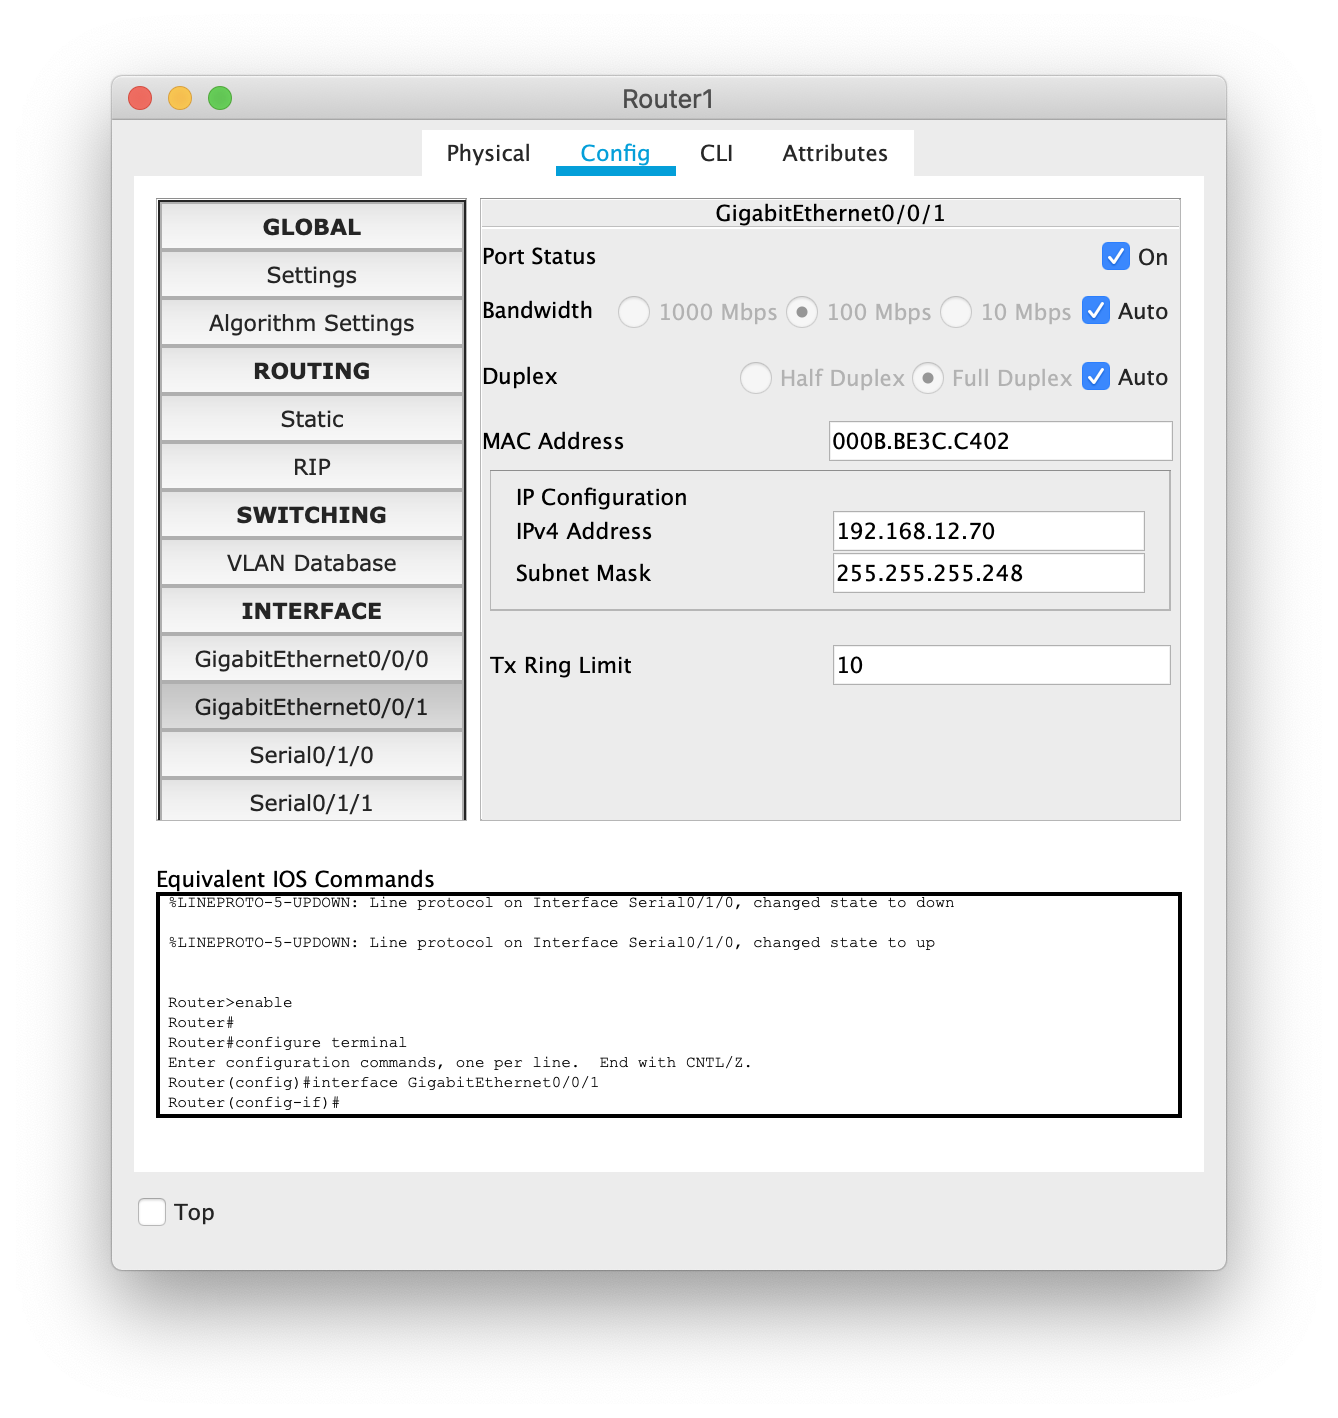
\includegraphics[width=0.8\linewidth]{images/router_1.png}
    \caption{Настройка маршрутизатора в роли DHCP-сервера для подсети №2}%
\end{figure}

\begin{figure}[H]
    \centering
    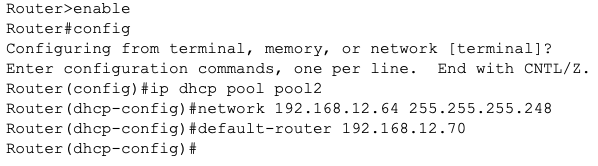
\includegraphics[width=0.8\linewidth]{images/router_1_conf.png}
    \caption{Настройка маршрутизатора}%
\end{figure}

IP-адреса конечным узлам в подсети выдаются автоматически из диапазона сетей подсети №2:

\begin{figure}[H]
    \centering
    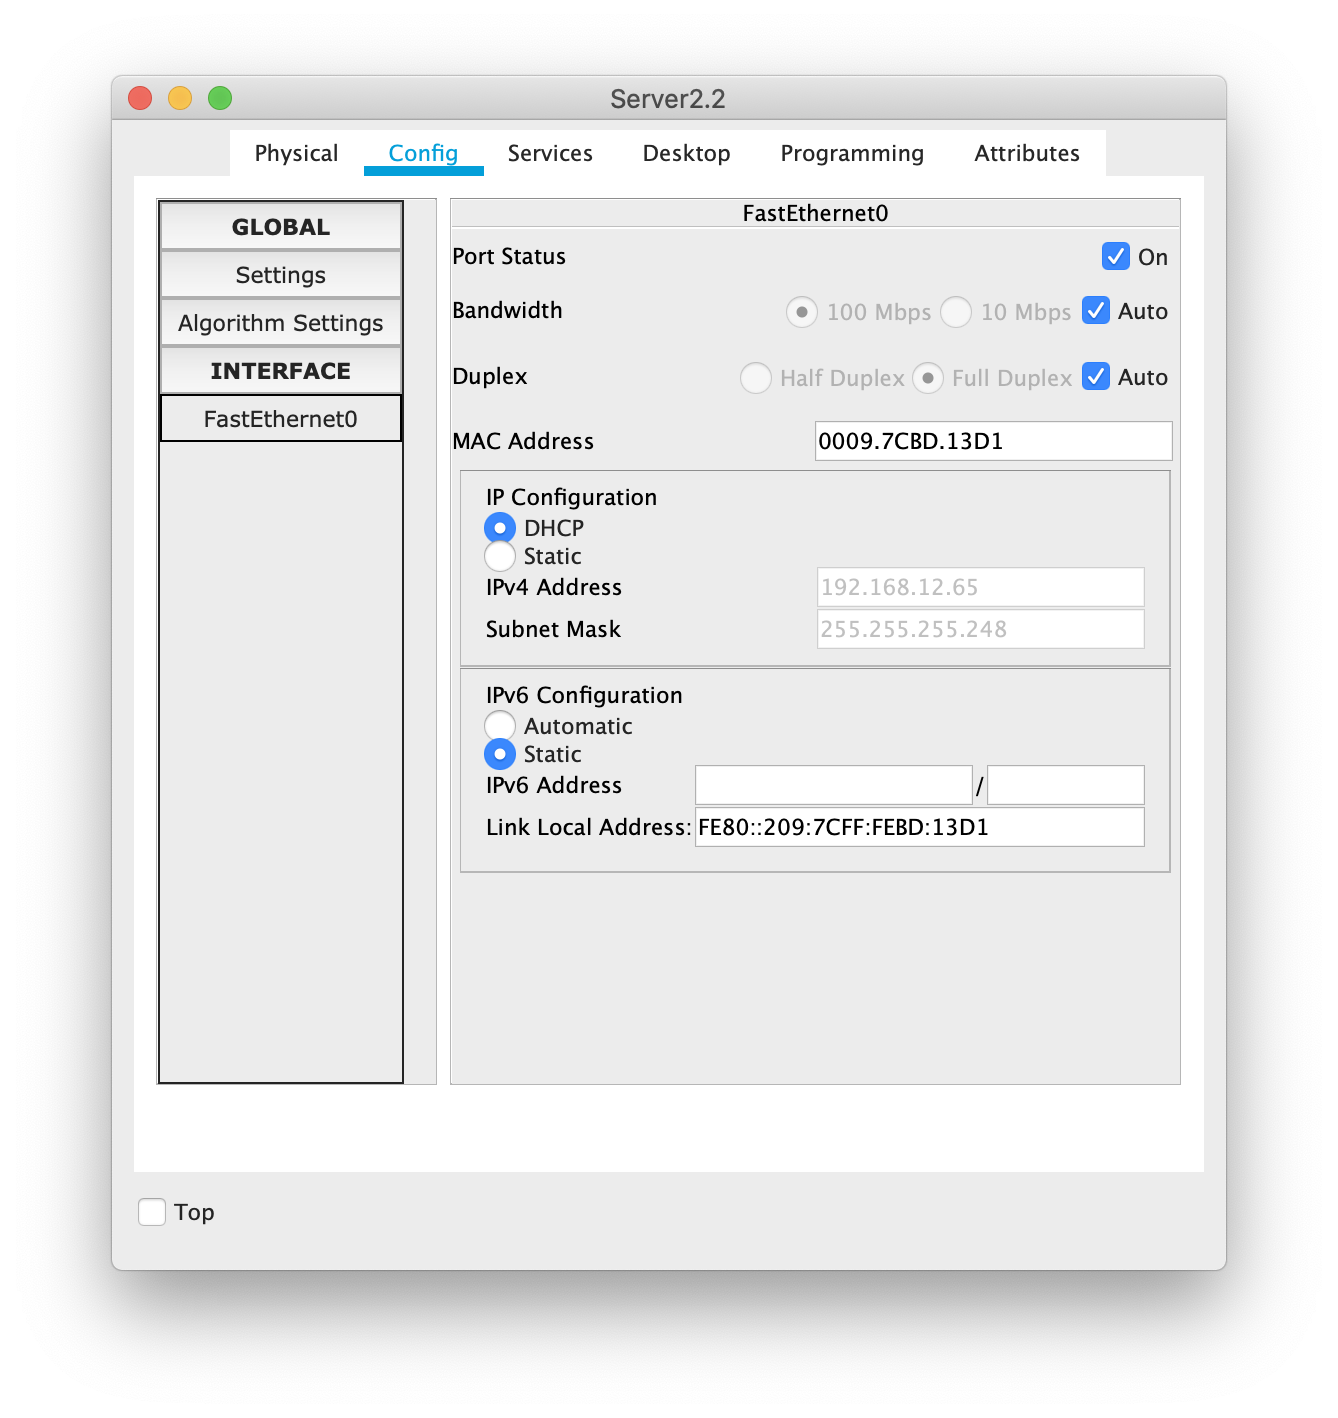
\includegraphics[width=0.7\linewidth]{images/net_2_machine.png}
    \caption{Автоматически выданный ip-адрес во второй подсети}%
\end{figure}


Проверка связи компьютеров в подсети №2:
\begin{figure}[H]
    \centering
    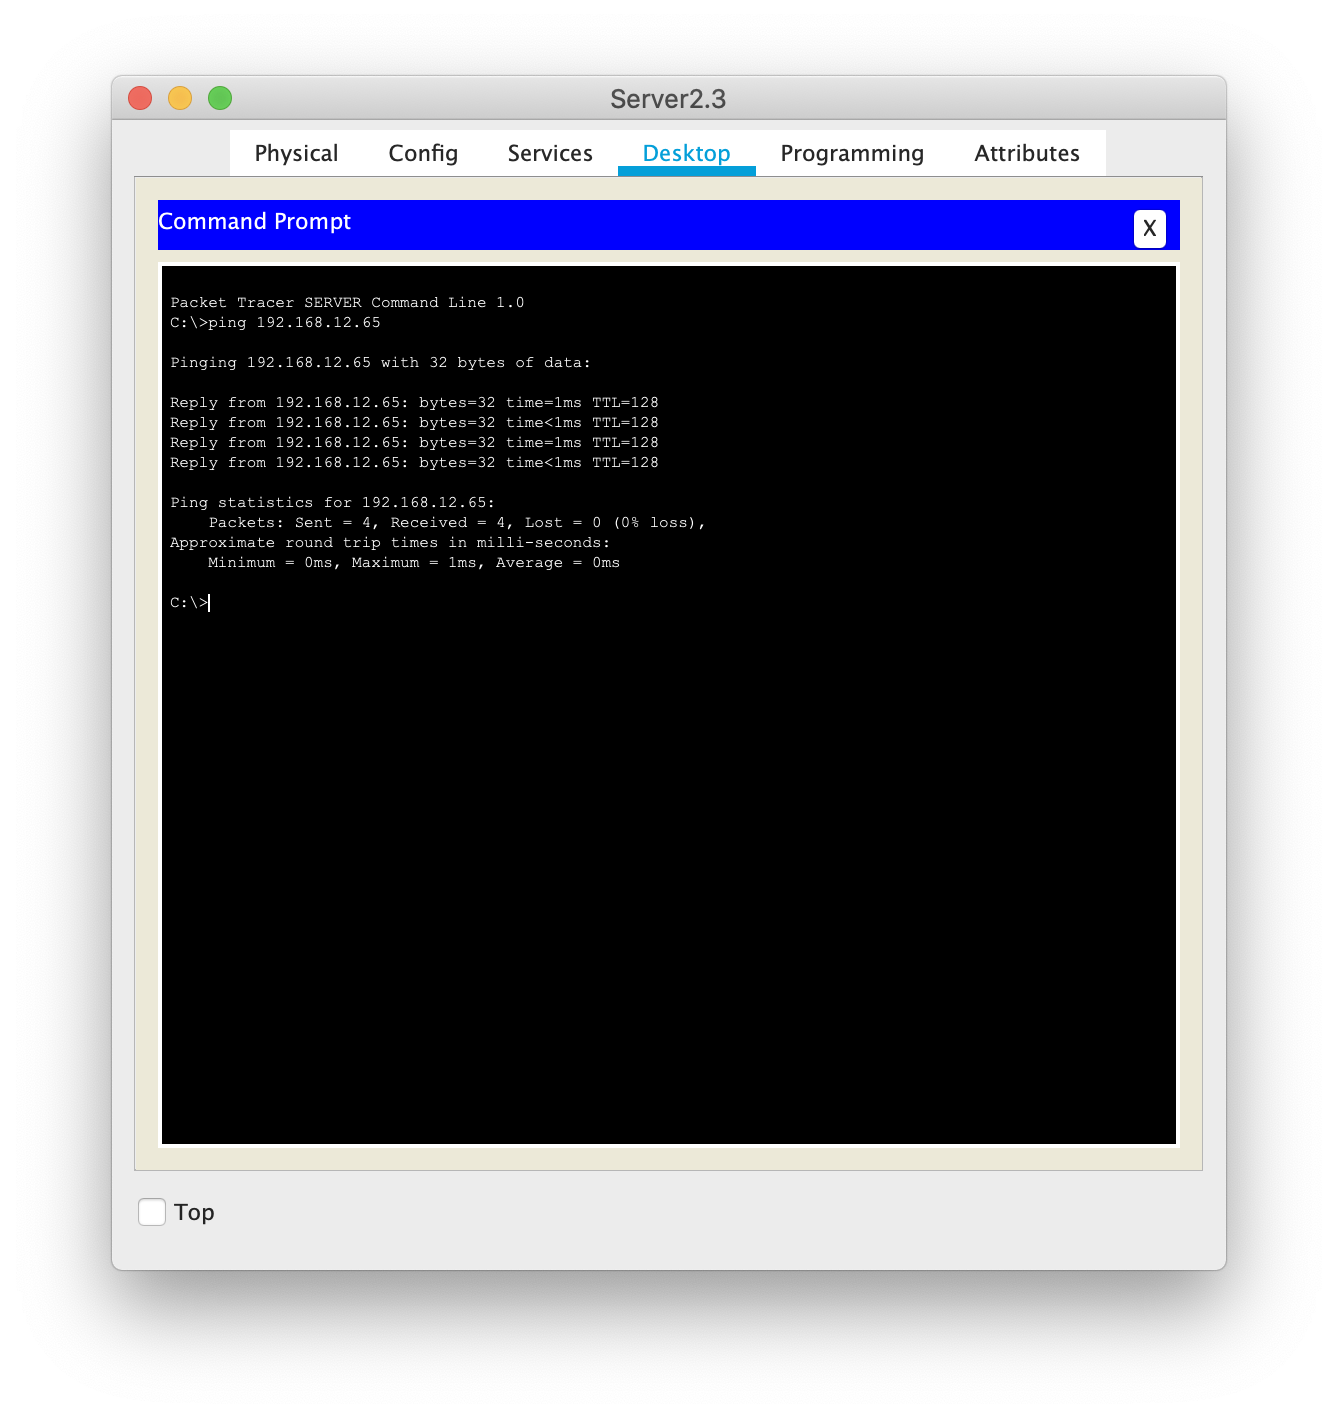
\includegraphics[width=0.8\linewidth]{images/net_2_ping.png}
    \caption{Результат использования ping}%
\end{figure}

\section{Настройка 3-ой подсети}%
\label{sec:3_net}
\begin{figure}[H]
    \centering
    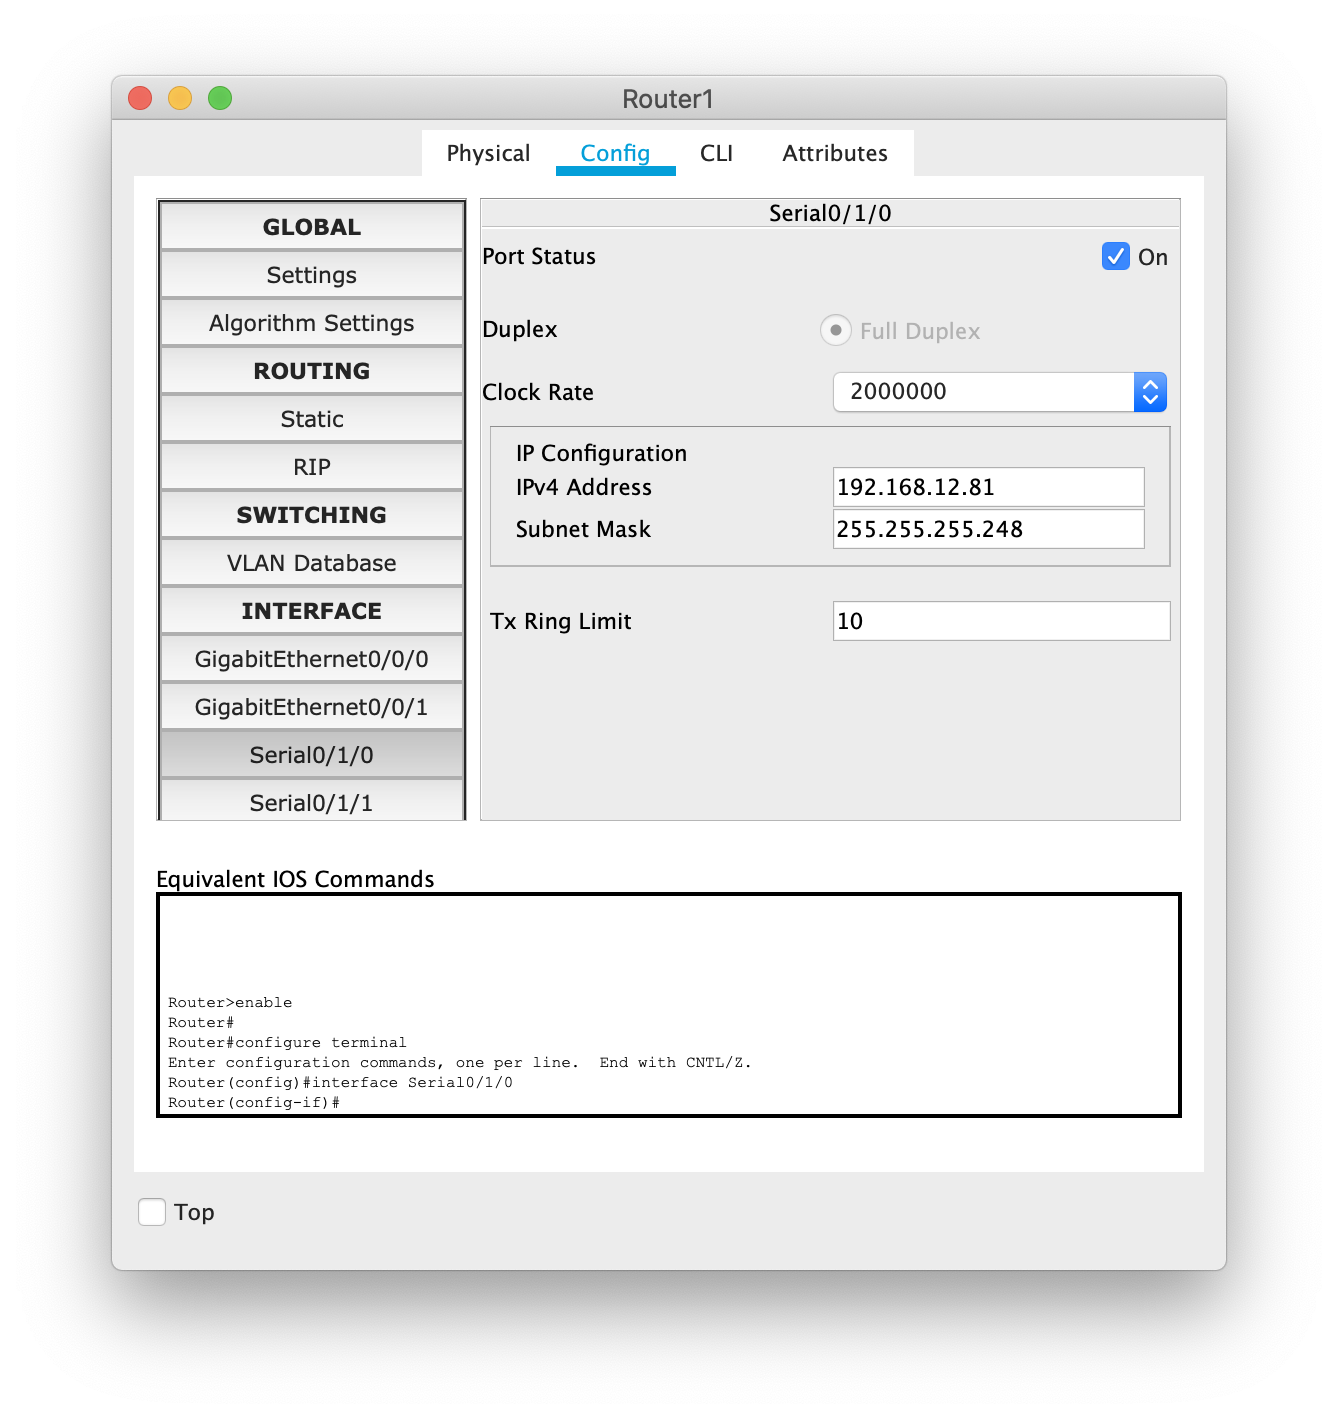
\includegraphics[width=0.8\linewidth]{images/net_3_1.png}
    \caption{Настройка первого маршрутизатора}%
\end{figure}

\begin{figure}[H]
    \centering
    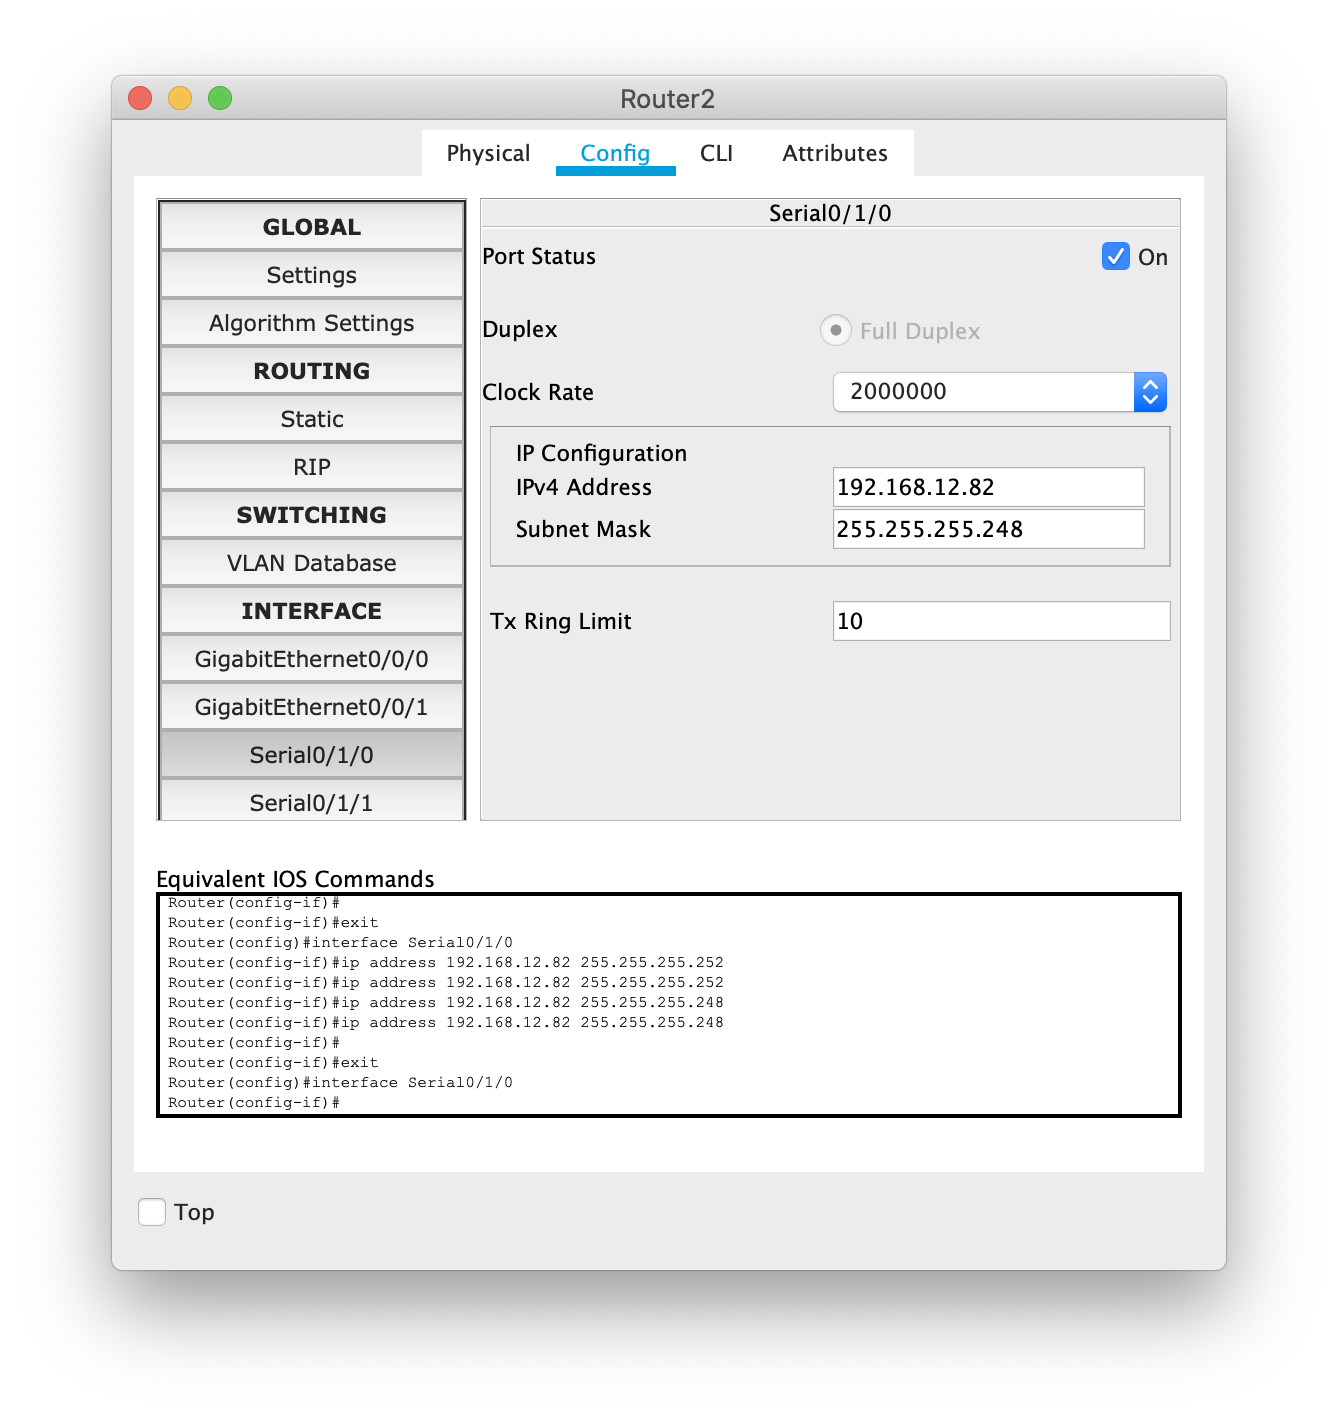
\includegraphics[width=0.8\linewidth]{images/net_3_2.png}
    \caption{Настройка второго маршрутизатора}%
\end{figure}

\section{Настройка DHCP-сервера для 4-ой подсети}%
\label{sec:4_net}
\begin{figure}[H]
    \centering
    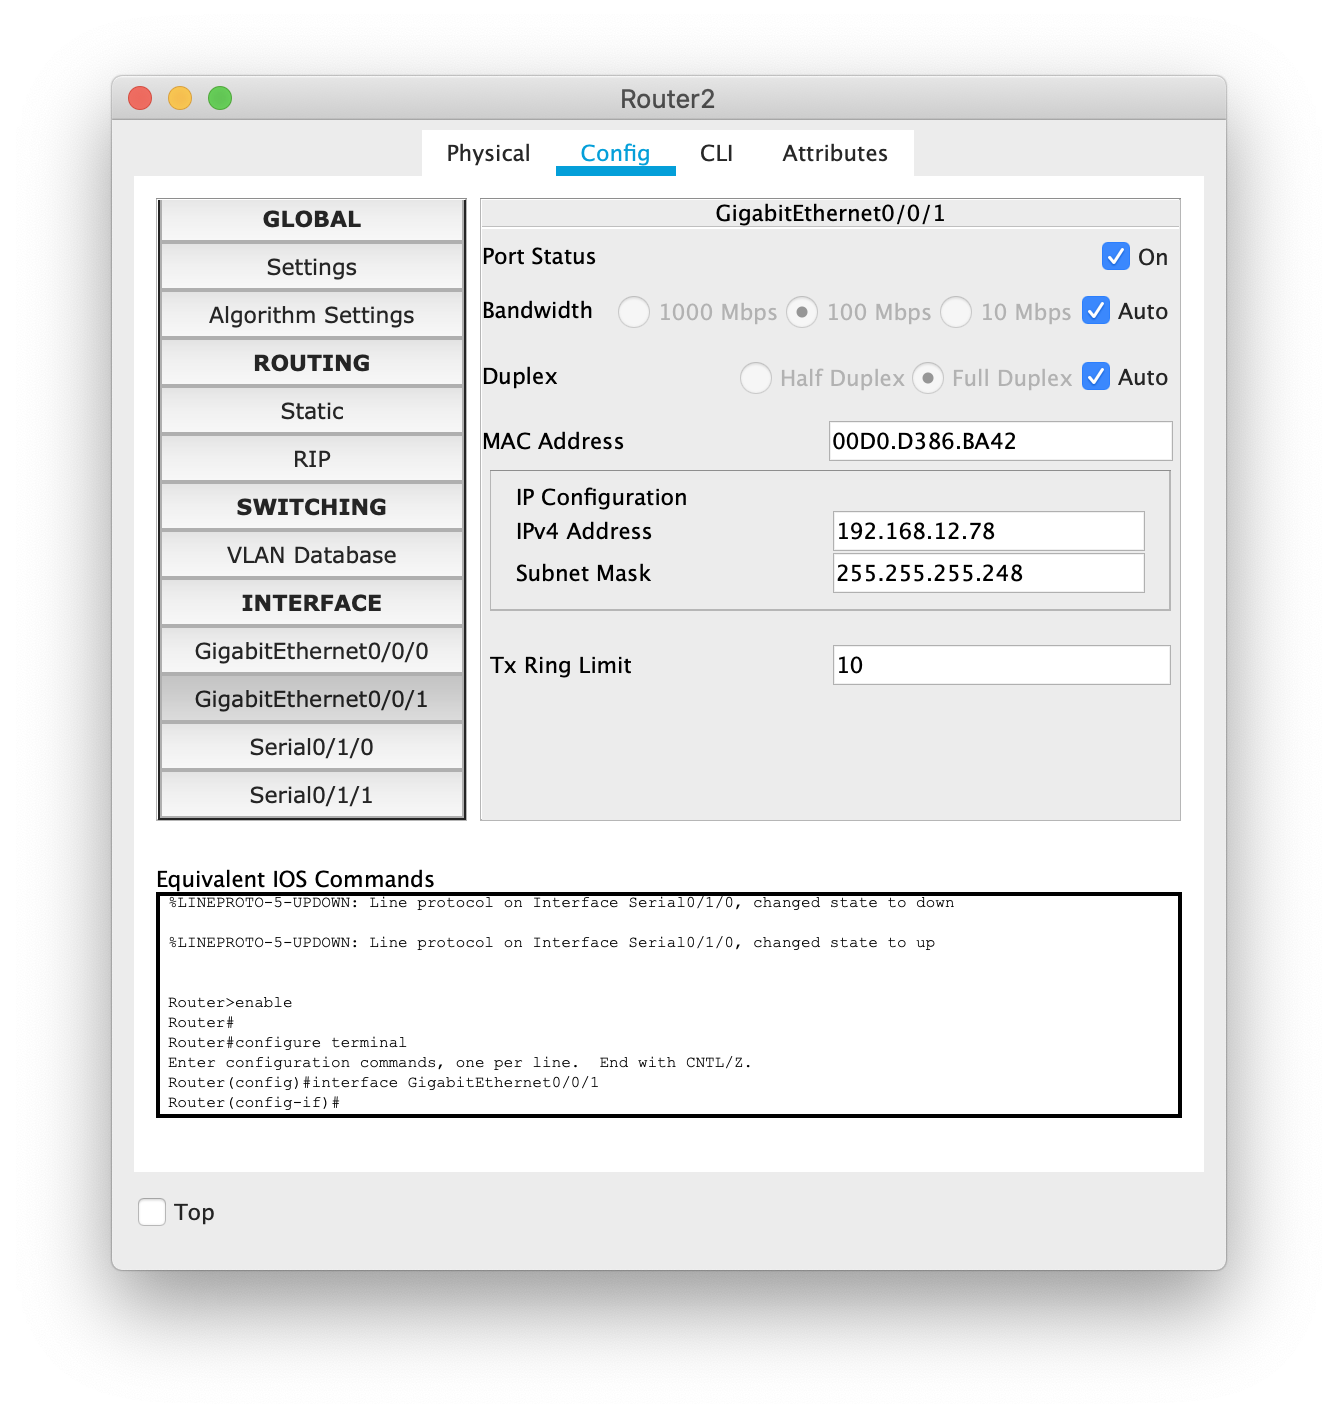
\includegraphics[width=0.8\linewidth]{images/router_2.png}
    \caption{Настройка маршрутизатора в роли DHCP-сервера для подсети №4}%
\end{figure}

\begin{figure}[H]
    \centering
    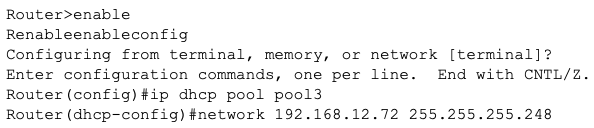
\includegraphics[width=0.8\linewidth]{images/router_2_conf.png}
    \caption{Настройка маршрутизатора}%
\end{figure}

IP-адреса конечным узлам в подсети выдаются автоматически из диапазона сетей подсети №4:

\begin{figure}[H]
    \centering
    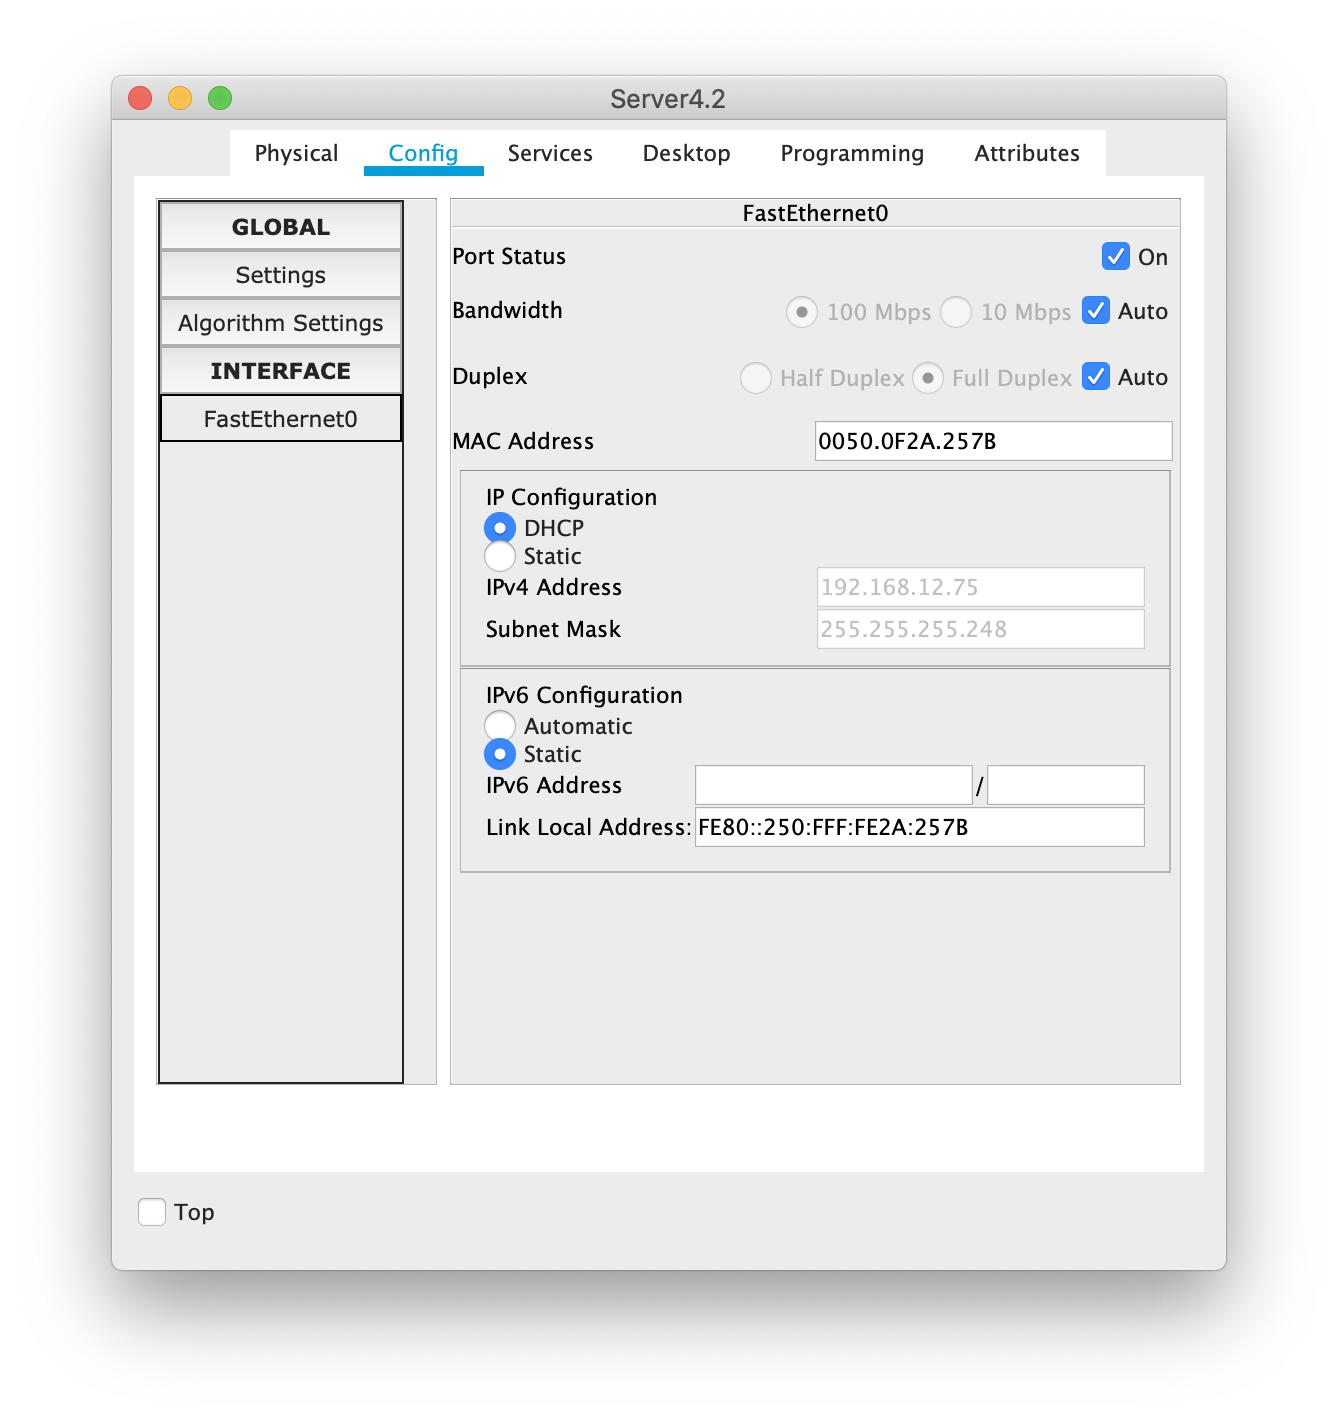
\includegraphics[width=0.7\linewidth]{images/net_4_macine.png}
    \caption{Автоматически выданный ip-адрес в подсети №4}%
\end{figure}

\section{Настройка DHCP-сервера для 5-ой подсети}%
\label{sec:4_net}

\begin{figure}[H]
    \centering
    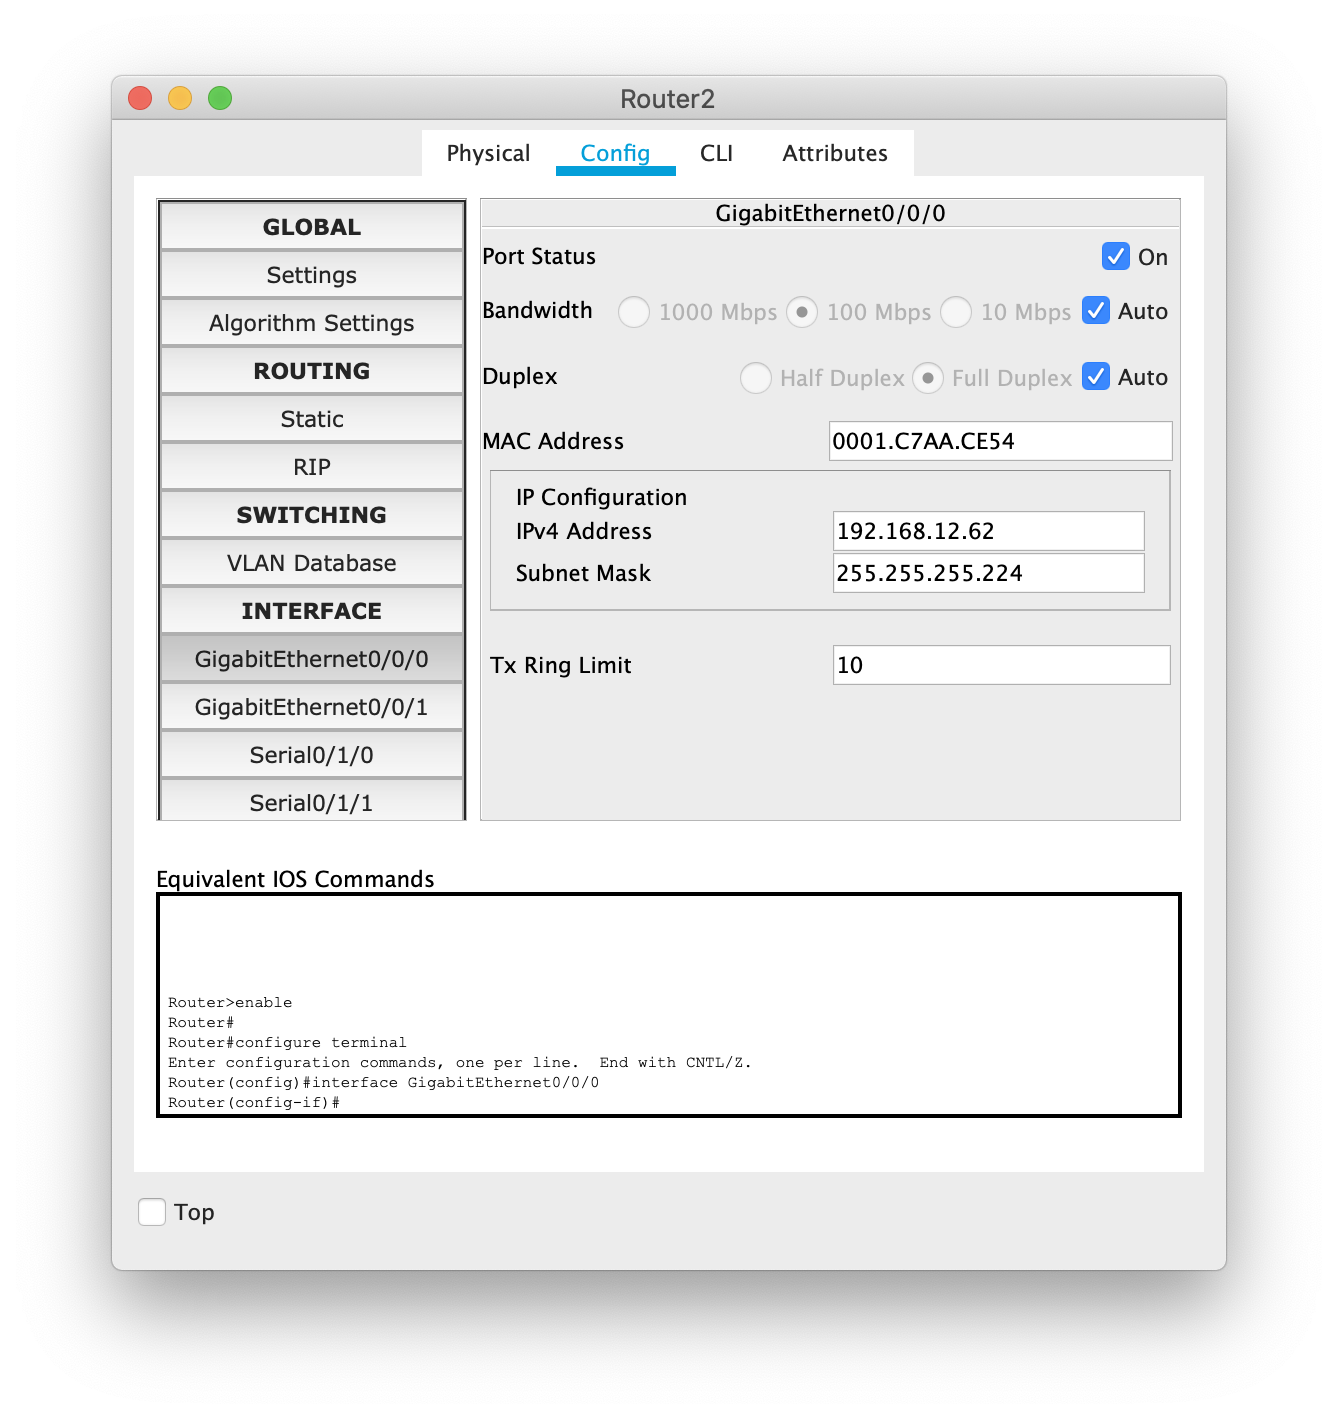
\includegraphics[width=0.8\linewidth]{images/router2_net_5.png}
    \caption{Настройка маршрутизатора в роли DHCP-сервера для подсети №5}%
\end{figure}

\begin{figure}[H]
    \centering
    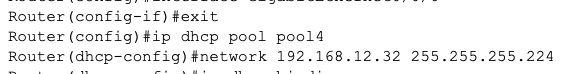
\includegraphics[width=0.8\linewidth]{images/net_5.png}
    \caption{Настройка маршрутизатора}%
\end{figure}

\begin{figure}[H]
    \centering
    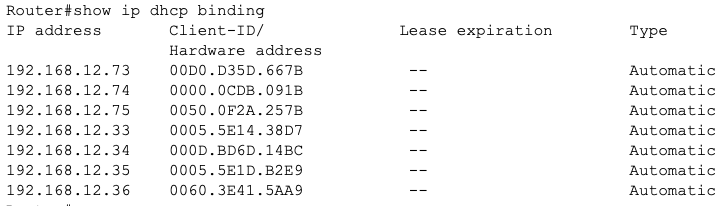
\includegraphics[width=0.8\linewidth]{images/net_4_5.png}
    \caption{Результат использования show ip dchp binding}%
\end{figure}

IP-адреса конечным узлам в подсети выдаются автоматически из диапазона сетей подсети №5:

\begin{figure}[H]
    \centering
    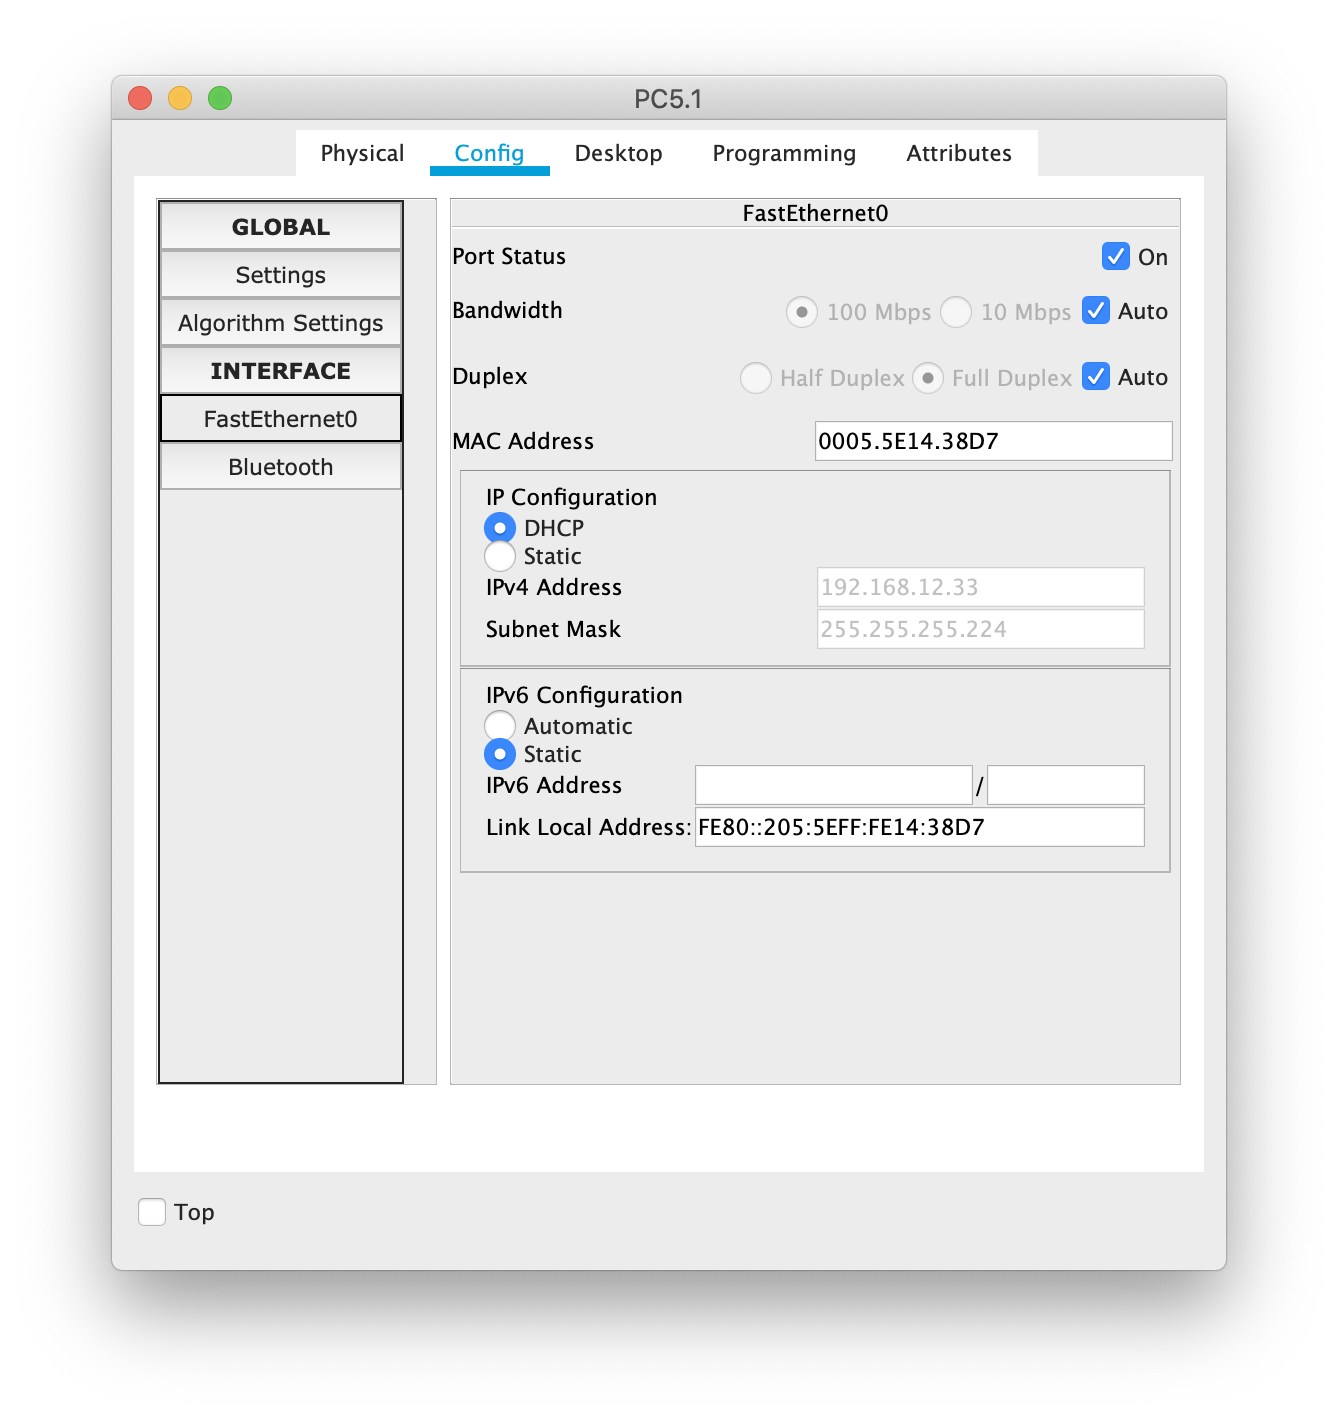
\includegraphics[width=0.7\linewidth]{images/net_5_machine.png}
    \caption{Автоматически выданный ip-адрес в подсети №5}%
\end{figure}

\chapter{Проверка с помощью ping}%
\label{cha:vyvod}

На рисунке ниже представлен примеры работы команды pind.

В первый раз происходит подключение в рамках одной подсети, а во второй происходит попытка подключения к адресу из другой подсети.

Попытка подключения в одной подсети:
\begin{figure}[H]
    \centering
    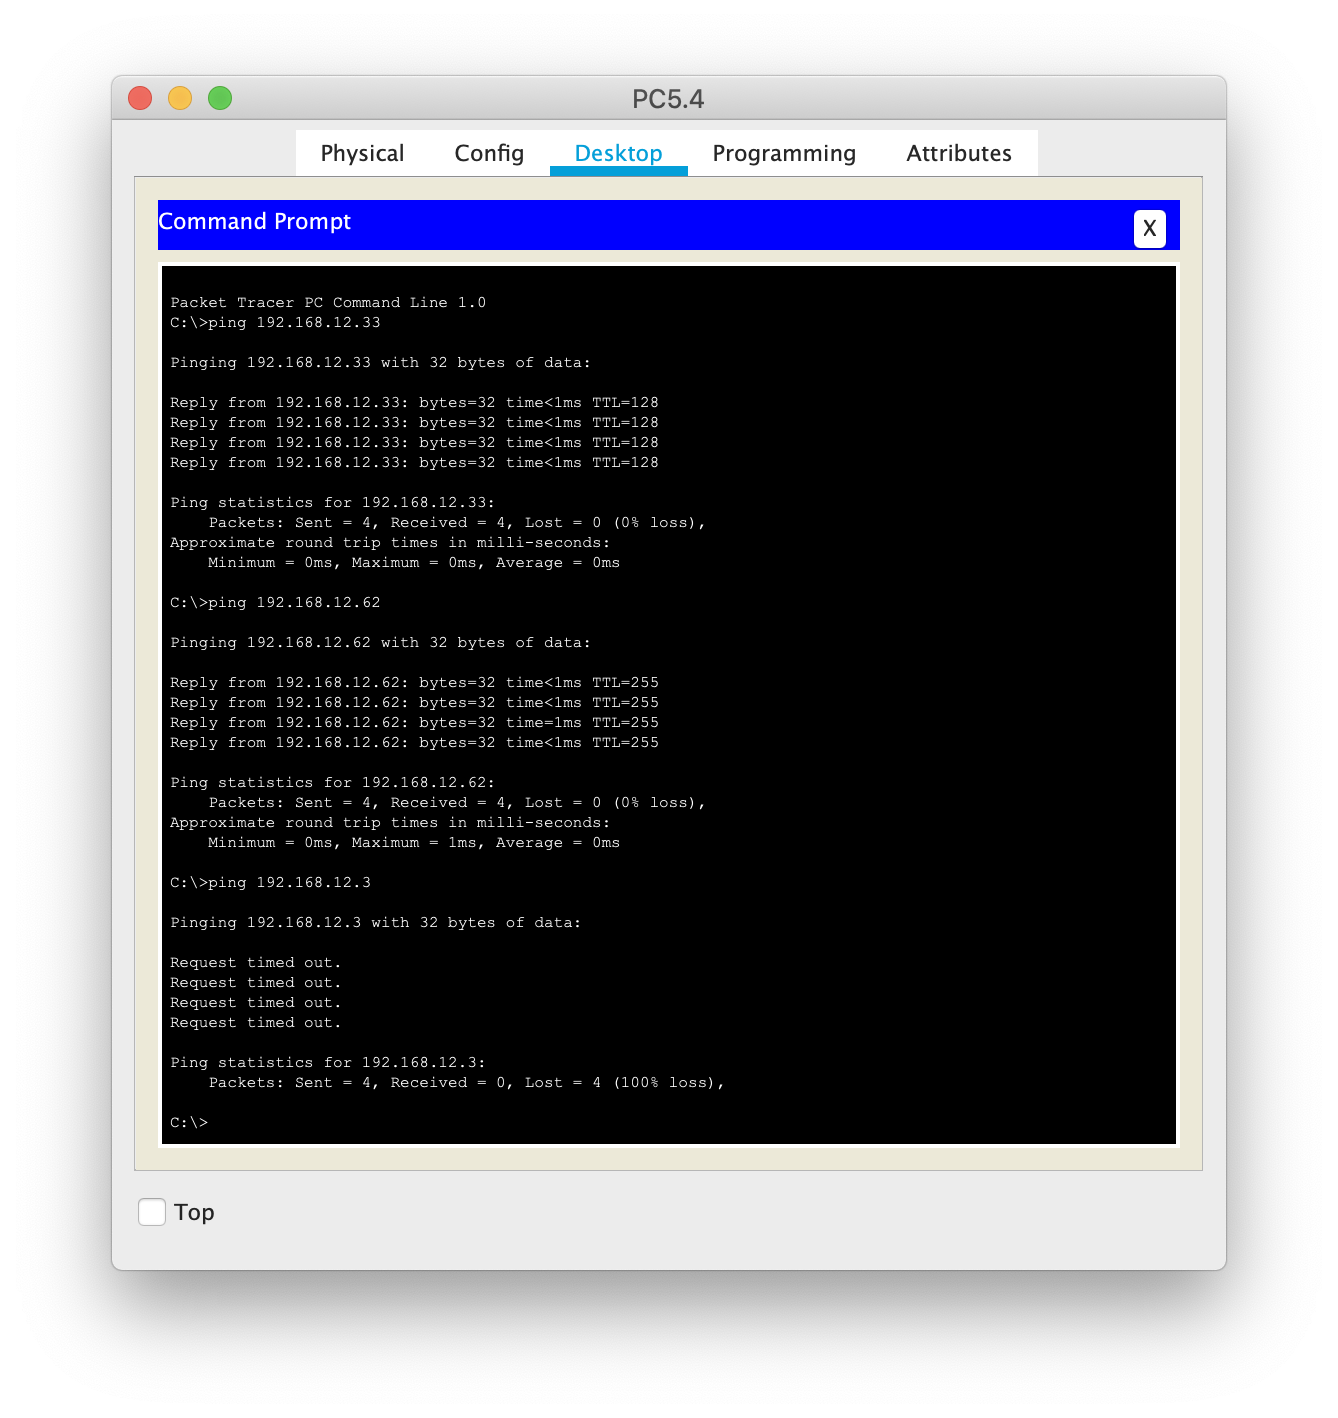
\includegraphics[width=0.7\linewidth]{images/ping_1.png}
    \caption{Результат работы ping}%
\end{figure}

